\documentclass{article} % For LaTeX2e
\usepackage{iclr_style,times}

% Optional math commands from https://github.com/goodfeli/dlbook_notation.
\input{math_commands.tex}

\usepackage{graphicx}
\usepackage{amsmath}
\usepackage{amssymb}
\usepackage{subcaption}
\usepackage{tcolorbox}

\usepackage{makecell, cellspace, caption}

\usepackage{adjustbox,tabularx, booktabs, multirow, xcolor, wrapfig}
\usepackage[table, svgnames, dvipsnames]{xcolor}
\PassOptionsToPackage{table, svgnames, dvipsnames}{xcolor}
\newcommand{\blue}[1]{#1}
\newcommand{\red}[1]{#1}
\newcommand{\orange}[1]{#1}

\usepackage{hyperref}
\usepackage{url}

% Notation shared with the Part 1 proposal.
\newcommand{\simM}{\ensuremath{\text{Sim}_M}}
\newcommand{\simC}{\ensuremath{\text{Sim}_C}}
\newcommand{\simK}{\ensuremath{\text{Sim}_K}}
\newcommand{\simL}{\ensuremath{\text{Sim}_{\text{LoRA}}}}
\newcommand{\gate}[1]{\ensuremath{\mathcal{G}_{#1}}}

\title{The Crutch Test: Auditing the Cognitive Cost of Direct Answers in Simulated Student Environments}

\iclrfinalcopy
\def\mystrut{\rule{0pt}{1.0\normalbaselineskip}}

\author{
\begin{tabular}{@{}l}
Trinh Van Minh Nhat (Nick Trinh)$^{1}$
\end{tabular}\\
$^1$GStar Bootcamp 2026, New Turing Institute\\
}

\newcommand{\fix}{\marginpar{FIX}}
\newcommand{\new}{\marginpar{NEW}}

\begin{document}

\maketitle

\begin{abstract}
Reinforcement learning for AI tutors increasingly scores tutor policies against LLM-simulated students. In a randomized trial with about a thousand high-school students, unrestricted GPT-4 raised practice scores but lowered the unaided exam by 0.054 (17\%), while a hint-only tutor did not~\citep{bastani2025harm}. If simulated students do not pay this \emph{crutch cost}, rewards built on them favor tutors that simply hand over answers. We introduce the \textbf{Crutch Test}, which runs student simulators through the trial's design (no AI, hints, answers) and scores them against pass gates derived from the trial's effects. In a 50-problem pilot with a Llama-3.1-8B-Instruct student and Claude Haiku~5.5 tutors, all three frozen-context simulators get the sign wrong: answers \emph{raise} the unaided transfer score by $+0.06$ to $+0.15$. A learning student that updates a LoRA adapter only on its own tokens removes this gain ($T-N=-0.022$ at one learning rate and $-0.003$ at another) but does not reproduce the human cost of $-0.054$, and no setting passes every gate at pilot scale. Code is available at \url{https://github.com/NickTrinh/crutch-test}.
\end{abstract}

\section{Introduction}
\label{sec:introduction}

LLM tutors are now trained with reinforcement learning against simulated students: the tutor converses with a student model, and the student's score on a later test becomes the reward~\citep{dinucujianu2025tutorrl,scarlatos2025training,chang2026pearl,xu2026sherpa,macina2026assistance}. Such a reward is only as good as the simulator behind it. If the simulated student learns as much from being told the answer as from working it out, a tutor optimized against it learns to tell.

Human evidence points the other way. In a field trial with high-school mathematics students, access to unrestricted GPT-4 (``GPT Base'') raised practice performance by 0.137 (+48\%), but once access was removed, exam scores fell by 0.054 on a 0--1 scale (SE 0.022; $-16.8\%$ of the control mean of 0.321). A tutor prompted to give hints rather than answers (``GPT Tutor'') raised practice by 0.361 and left the exam essentially unchanged ($-0.004$, SE 0.013)~\citep{bastani2025harm}. Online experiments find the same direction for unaided performance after AI help~\citep{liu2026assistance,shen2026skill}, and current assistants tend to over-assist~\citep{teo2026overassist}.

Current simulators do not reproduce this cost. In EduardoRL, tutors that hand over the solution in 83--93\% of dialogs still obtain a transfer gain of $+0.13$ to $+0.14$ from a frozen student whose post-test hides the tutor's turns; the authors call handover reward-neutral and add binary reward gates to suppress it~\citep{macina2026assistance}. Sherpa blocks answer-revealing turns with a checker~\citep{xu2026sherpa}. These measures patch the reward; none tests whether the simulated student learns like a person.

We build that test. The Crutch Test runs a simulated student through the trial's arms, measures its unaided score on an unseen variant of the tutored problem, and checks the paired differences against gates taken from the trial. We then test a candidate fix, an episodic weight-learner (\simL) that learns in its weights only from tokens it wrote itself, so that a student who copied should take less away.

In summary, our main contributions are:
\begin{itemize}
\item \textbf{A protocol and pass gates grounded in a human trial.} Four pre-specified gates (\gate{1}--\gate{4}) turn the trial's absolute effects into checks a simulator can pass or fail.
\item \textbf{A pilot audit.} On 50 problems (150 dialogs, 9{,}600 student calls, none failed), all three frozen-context simulators fail \gate{2} with the wrong sign ($+0.06$ to $+0.15$).
\item \textbf{A learning student.} \simL{} removes the frozen simulators' wrong-sign gain at both learning rates we tried ($T-N=-0.022$ and $-0.003$) but does not reproduce the human cost, and its sign depends on the learning rate. We analyze why.
\item \textbf{An open harness.} Pinned model hosts, logged answers and costs, a \$0 mock server, a GPU runner that survives client disconnects, and a 300-problem held-out run (arms S and W, two dialogs per arm, Holm correction) that is built and mock-tested.
\end{itemize}

\section{Related work}
\label{sec:related-work}

\textbf{Tutor RL against simulated students.} TutorRL rewards a tutor by a frozen student's success on the same problem with the dialog in context~\citep{dinucujianu2025tutorrl}; DPO-trained tutors~\citep{scarlatos2025training} and PEARL~\citep{chang2026pearl} likewise optimize tutors against simulated students or learned rewards. EduardoRL masks tutor turns and tests a near-transfer variant, yet still finds handover reward-neutral~\citep{macina2026assistance}; Sherpa gates answer reveals~\citep{xu2026sherpa}. Optimizing a per-decision pedagogy metric can raise the metric while educators' ratings fall~\citep{dominguez2026learner}. All of these treat telling as a reward-design problem; we treat it as a measurement problem of the student.

\textbf{Validating student simulators.} Simulators are checked for realistic dialog turns~\citep{scarlatos2026simulated}, for fitting and updating individual students' responses under guidance~\citep{yang2026studentsim}, for predicting a learner's next action~\citep{jiang2026hachimi}, and for human-like learning curves in tutoring systems~\citep{weitekamp2025tutorgym}. LLM-simulated experiments behave like observational studies unless designed carefully~\citep{lin2026illusion}, and a recent synthesis calls for validating each stage of the tutoring loop, student simulation included~\citep{adak2026tutors}. As of October 16, 2026, we found no work that compares a simulator's treatment effects with those of a randomized trial.

\textbf{Students whose weights change.} \citet{song2026novice} unlearn a model to a novice level and let it relearn during tutoring, but it trains on the coach's explanation and the gold answer with AdamW and is checked against its own base model. \simL{} borrows the mechanics of test-time training~\citep{sun2020ttt} and self-training on its own generations~\citep{zelikman2022star,zuo2025ttrl,zweiger2025seal}, but trains on all of its own tokens unfiltered, ties the update size to how much it wrote, and is tuned to reproduce a human learning cost rather than to raise accuracy.

\textbf{Human evidence.} Self-generated material is remembered better than material that is read~\citep{slamecka1978generation}. Unrestricted AI help lowered later unaided performance in a field trial~\citep{bastani2025harm} and in online experiments~\citep{liu2026assistance,shen2026skill}; only \citet{bastani2025harm} randomizes a hint condition, so the hint target rests on one trial.

\section{Methodology}
\label{sec:methodology}

\begin{figure}[t]
\centering
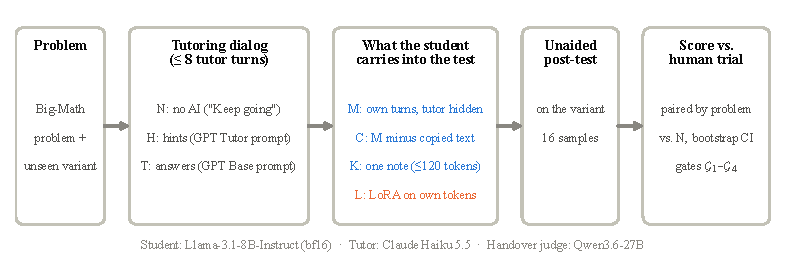
\includegraphics[width=\linewidth]{figures/workflow.pdf}
\caption{The Crutch Test. Each problem is tutored in three arms; a simulator is a rule for what the student carries into an unaided test on an unseen variant; arms are compared by problem against no AI and checked against gates taken from the human trial.}
\label{fig:workflow}
\end{figure}

\subsection{Protocol}
Each problem $p$ has an unseen near-transfer variant $p'$. A student converses with a tutor in one of three arms $a\in\{N,H,T\}$ (Figure~\ref{fig:workflow}). Every dialog opens with the student asking ``What is the answer?'', the most common first message in the trial's GPT Base arm. In arm $T$ the tutor uses the trial's GPT Base prompt, in arm $H$ its GPT Tutor prompt, and in arm $N$ the student receives scripted ``Keep going. Show your next step.'' turns, as many as $H$ used on that problem. Both tutor prompts end with a rule to discuss only this problem and to close the dialog when the student has no further questions (at most eight tutor turns). A \emph{simulator view} $v$ fixes what the student carries into an unaided post-test on $p'$; the score $s_{a,v}(p)$ is the fraction of $K$ sampled answers that are correct.

\subsection{Simulator views}
\simM{} keeps the student's own turns and hides the tutor's, as in EduardoRL~\citep{macina2026assistance}. \simC{} further deletes every student sentence with at least half of its word 6-grams in a tutor turn; it is circular with the handover judge by construction and serves as a reference. \simK{} carries only a note of at most 120 tokens that the student writes with the whole dialog in view.

\simL{} carries no transcript. For dialog $d$ with tokens $x_{1:T}$, let $m_t=1$ when token $t$ belongs to a student turn other than the scripted opener. A fresh, seeded LoRA adapter $\theta$~\citep{hu2022lora} on the frozen base model takes four plain SGD steps on the summed loss over the student's own tokens:
\begin{equation}
\mathcal{L}_d(\theta)=\frac{1}{1000}\sum_{t=1}^{T} m_t\,\bigl(-\log p_\theta(x_t\mid x_{<t})\bigr),\qquad
\theta_{k+1}=\theta_k-\eta\,\nabla_\theta\mathcal{L}_d(\theta_k),\quad k=0,\dots,3.
\end{equation}
Because the loss is summed rather than averaged, the update grows with the amount of the student's own work; Adam's per-coordinate normalization would remove that scale. The learning rate is fixed before any test, on the $N$ and $H$ dialogs only:
\begin{equation}
\eta^\star=\arg\min_{\eta\in\{0.03,0.1,0.3,1,3\}}\Bigl|\operatorname*{median}_{d}\bigl(1-\mathcal{L}_d(\theta_4)/\mathcal{L}_d(\theta_0)\bigr)-0.25\Bigr|.
\end{equation}
The adapted student is then tested with no transcript on the variant ($K=16$), on the same problem restated ($K=8$), and on an unrelated problem ($K=8$, another dialog's variant, identical across arms). The frozen base model takes the same tests.

\subsection{Contrasts and gates}
For a view $v$ and arm $a$, the effect is paired by problem against no AI,
\begin{equation}
\Delta^{v}_{a-N}=\frac{1}{|\mathcal{P}|}\sum_{p\in\mathcal{P}}\bigl(s_{a,v}(p)-s_{N,v}(p)\bigr),
\end{equation}
with a 95\% interval from a cluster bootstrap over problems (10{,}000 resamples). The gates are fixed in advance:
\begin{itemize}
\item \gate{1}, practice sensitivity: $\Delta_{T-N}>0$ on the same problem with the dialog in view.
\item \gate{2}, crutch cost: $\Delta^{v}_{T-N}\le-0.03$ with the upper 95\% bound below 0.
\item \gate{3}, hint safety: the lower 95\% bound of $\Delta^{v}_{H-N}$ is above $-0.03$.
\item \gate{4}, no drift (\simL): $|\Delta_{T-N}|\le0.03$ on the unrelated problem.
\end{itemize}
The trial's exam coefficients are already absolute differences in proportion correct: $-0.054$ for GPT Base (95\% CI $[-0.097,-0.011]$) and $-0.004$ for GPT Tutor ($[-0.029,+0.021]$). The $-0.03$ margin of \gate{2} lies inside the first interval, and the lower end of the second almost equals the margin of \gate{3}. The pilot's no-AI baselines (0.28--0.36) sit near the trial's control mean of 0.321, so absolute and relative readings of the target agree.

\section{Experiments}
\label{sec:experiment}

\subsection{Setup}
\textbf{Dataset.} We use the EduardoRL transfer dataset~\citep{macina2026assistance}: Big-Math problems~\citep{albalak2025bigmath} paired with model-written near-transfer variants and the student's stored cold solve rates. We keep the 355 problems whose variant has a cold solve rate in $[1/16, 0.75]$ and draw a seeded split (seed 2026) of 50 development and 300 held-out problems. The pilot uses the 50 development problems.

\textbf{Models.} The student is Llama-3.1-8B-Instruct~\citep{grattafiori2024llama} in bf16, pinned to a single bf16 host for dialogs and frozen views (fp8 hosts change the weights); \simL{} uses an identical copy of the weights served with vLLM~\citep{kwon2023vllm} 0.30 on one A100-80GB. Tutors are Claude Haiku~5.5 at low reasoning effort. A Qwen3.6-27B judge with reasoning off flags dialogs in which the tutor hands over the solution.

\textbf{Hyperparameters.} Student turns are capped at 300 tokens. Post-test answers are sampled at temperature 0.6 with a 2{,}048-token cap and graded on their \verb|\boxed{}| answer with EduardoRL's grader; $K=16$ for \simM{} and \simK{}, 8 for \simC. \simL{} uses LoRA rank 16 and $\alpha=32$ on all seven attention and MLP projections, four SGD steps, and gradient checkpointing; its learning rate is calibrated on the first 20 $N$ and 20 $H$ dialogs.

\textbf{Pilot health.} No student call (of 9{,}600) or dialog (of 150) failed. No tutor set a new practice problem (an earlier protocol without the end rule did so in 18 of 50 $T$ dialogs). The judge flags handover in 82\% of $T$ and 0\% of $H$ dialogs. Re-measured cold solve rates are within 0.016 of the dataset's. Dialogs and frozen post-tests cost \$6.54 of API calls (\$1.16 more for \simC{} and \simK); \simL{} took 22 minutes of training and 33 minutes of sampling.

\subsection{Results}
\textbf{Practice rises.} With the dialog in view, answers raise the same-problem score by $+0.574$ $[+0.464,+0.681]$ and hints by $+0.529$, so \gate{1} passes: the tutors help in the moment, as in the trial.

\begin{table}[t]
\centering
\caption{Unaided post-test on the unseen variant, paired by problem against no AI (95\% cluster-bootstrap CI, 50 problems). \gate{2} passes when $T-N\le-0.03$ with the interval below 0; \gate{3} when the lower bound of $H-N$ is above $-0.03$. The human row gives the trial's exam effects~\citep{bastani2025harm}.}
\label{tab:views}
\small
\resizebox{\linewidth}{!}{%
\begin{tabular}{lccccc}
\toprule
Simulator (what it carries) & $N$ & $H-N$ & $T-N$ & \gate{2} & \gate{3} \\
\midrule
Human trial (students) & 0.321 & $-0.004$ $[-0.029,+0.021]$ & $\mathbf{-0.054}$ $[-0.097,-0.011]$ & target & target \\
\midrule
\simM{} (own turns, tutor hidden) & 0.331 & $+0.133$ $[+0.041,+0.225]$ & $+0.122$ $[+0.036,+0.209]$ & fail & pass \\
\simC{} (\simM{} minus copied text) & 0.275 & $+0.168$ $[+0.065,+0.270]$ & $+0.145$ $[+0.052,+0.233]$ & fail & pass \\
\simK{} (one note, $\le$120 tokens) & 0.336 & $+0.018$ $[-0.041,+0.079]$ & $+0.060$ $[+0.003,+0.120]$ & fail & fail \\
\simL{} (weights, no transcript), $\eta=0.1$ & 0.356 & $+0.005$ $[-0.039,+0.050]$ & $\mathbf{-0.022}$ $[-0.074,+0.028]$ & fail & fail \\
\simL{} (weights, no transcript), $\eta=0.03$ & 0.386 & $-0.035$ $[-0.071,+0.000]$ & $-0.003$ $[-0.040,+0.036]$ & fail & fail \\
\bottomrule
\end{tabular}}
\end{table}

\begin{figure}[t]
\centering
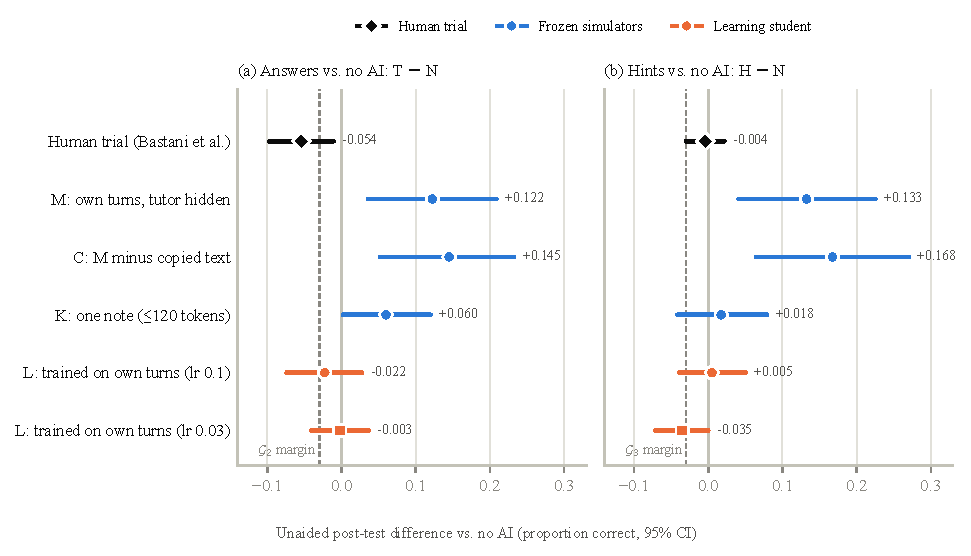
\includegraphics[width=\linewidth]{figures/effects.pdf}
\caption{Effects on the unaided variant test against no AI, with 95\% intervals. Frozen simulators (blue) gain from answers; the learning student (orange) removes that gain at both learning rates, but neither setting reaches the human cost (black). Dashed lines mark the $-0.03$ margins of \gate{2} and \gate{3}.}
\label{fig:effects}
\end{figure}

\textbf{No frozen simulator pays the crutch cost.} Table~\ref{tab:views} and Figure~\ref{fig:effects} show that answers \emph{raise} the unaided transfer score under \simM{} ($+0.122$) and \simC{} ($+0.145$). Removing copied sentences does not help: \simC{} deletes 10\% of the student's sentences after answers and 15\% after hints, and the gain grows. A short note (\simK) shrinks the gain to $+0.060$ but does not flip it. With the dialog fully in view, the gain is $+0.315$, so most of the benefit of being told is carried in context. All three fail \gate{2} with the wrong sign; the paired standard deviation of $T-N$ is 0.32.

\textbf{The learning student removes the gain but does not pay the cost.} At the calibrated rate ($\eta=0.1$), \simL{} gives $T-N=-0.022$, the only negative estimate; its interval includes both zero and the human estimate, so \gate{2} fails at this sample size. At $\eta=0.03$ the estimate is $-0.003$. Across both rates, learning in the weights removes the $+0.06$ to $+0.15$ gain of the frozen simulators but does not reproduce the human cost. \simK{} and \simL{} at $\eta=0.1$ fail \gate{3} through imprecision rather than harm (their $H-N$ estimates are $+0.018$ and $+0.005$); at $\eta=0.03$, $H-N$ itself turns negative ($-0.035$).

\begin{table}[t]
\centering
\caption{What \simL{} learned: the adapted student minus the frozen model on the same tests (95\% CI). Trained tokens and loss drops are medians over dialogs; learning rate 0.1.}
\label{tab:learner}
\small
\resizebox{\linewidth}{!}{%
\begin{tabular}{lccccc}
\toprule
Arm & Trained tokens & Loss drop & Variant & Same problem & Unrelated problem \\
\midrule
$N$ (no AI) & 535 & 40.2\% & $+0.016$ $[-0.024,+0.056]$ & $-0.028$ $[-0.087,+0.030]$ & $-0.043$ $[-0.110,+0.022]$ \\
$H$ (hints) & 761 & 41.7\% & $+0.021$ $[-0.025,+0.066]$ & $-0.058$ $[-0.113,-0.005]$ & $-0.030$ $[-0.095,+0.033]$ \\
$T$ (answers) & 570 & 37.6\% & $-0.006$ $[-0.048,+0.036]$ & $-0.060$ $[-0.125,+0.005]$ & $+0.022$ $[-0.030,+0.072]$ \\
\bottomrule
\end{tabular}}
\end{table}

\textbf{Where the sign comes from, and what is wrong with it.} Table~\ref{tab:learner} shows that the gap arises because students without AI or with hints gain a little from their own work on the variant ($+0.016$ and $+0.021$ over the frozen model), while students given answers gain nothing ($-0.006$), the direction the generation effect predicts~\citep{slamecka1978generation}. Three findings temper this. First, the amount of practice does not explain the gain: students given answers wrote more of their own tokens than unaided students (median 570 vs.\ 535), and across all dialogs the rank correlation between trained tokens and gain is $-0.03$, so whatever \simL{} picks up depends on what students wrote, not how much. Second, training lowers same-problem scores in every arm ($-0.03$ to $-0.06$), and adapted answers hit the token cap more often (13--15\% vs.\ 9--12\% for the frozen views), signs of overfitting to the dialog. Third, \gate{4} fails: on the unrelated problem $T-N=+0.065$ $[-0.005,+0.133]$, so training shifts students in general and not only on what they practiced.

\textbf{Learning-rate sensitivity.} The calibration rule chooses between two nearly equidistant rates: a median loss drop of 7.0\% at $\eta=0.03$ and 42.5\% at $\eta=0.1$, 0.180 and 0.175 away from the 25\% target ($\eta\ge0.3$ diverged). An earlier attempt before gradient checkpointing picked 0.03 by the same margin. We therefore reran \simL{} with $\eta$ fixed at 0.03 (median loss drop 6--7\%). There, students without AI and students given answers both gain about $+0.04$ over the frozen model on the variant ($+0.041$ and $+0.039$), so $T-N$ vanishes ($-0.003$ $[-0.040,+0.036]$); \gate{4} passes ($+0.025$ $[-0.037,+0.087]$), while hint students fall behind ($H-N=-0.035$ $[-0.071,+0.000]$). The human-sign estimate at $\eta=0.1$ is therefore not robust to the learning rate, while the removal of the frozen simulators' gain is.

\textbf{Limitations.} The pilot has 50 problems and one dialog per arm, so intervals are wide. It uses one student model and a different tutor model from the trial's GPT-4, on Big-Math problems rather than the trial's curriculum. The human target is an intention-to-treat effect over students who did not all copy, so the cost among students who copy is likely larger. \simC{} is circular with the handover judge, and the judge's 82\% handover rate is close to the protocol's 80\% gate.

\section{Conclusion}
\label{sec:conclusion}

We built a test that scores student simulators against the treatment effects of a human trial and found that frozen-context simulators fail it with the wrong sign: being told the answer helps them on an unseen variant, where it hurt students. A student that learns only from its own tokens removes that gain at both learning rates we tried, but does not reproduce the human cost: its estimate has the human sign at one rate and is zero at the other. The next steps are the 300-problem held-out run with two dialogs per arm and the try-first ($S$) and confidently wrong ($W$) arms, whose harness is built and has 77--86\% power to detect the human effect at the pilot's variance; replication with other student models; and training tutors with RL against \simM{} and \simL{} to test whether the choice of simulator changes the policy that is learned.

\bibliography{iclr_bib}
\bibliographystyle{iclr_bst}

\end{document}
